%
% .tex file needs 6_17.jpg, 6_19.jpg, and F6_26.jpg
%

\documentclass[12pt,letterpaper,boxed]{hmcpset}
\usepackage[margin=1 in]{geometry}
\usepackage{graphicx}
\usepackage{courier}
\usepackage{tabto}
\usepackage{amsmath, amssymb}
\usepackage{subfig}
\usepackage{framed}
\usepackage{enumerate}
\usepackage{pdfsync}
\usepackage{mathtools}
\usepackage{caption}
\usepackage{booktabs}
\usepackage{listings}
\usepackage{siunitx, xfrac}
\usepackage{color}



\definecolor{mygreen}{rgb}{0,0.6,0}
\definecolor{mygray}{rgb}{0.5,0.5,0.5}
\definecolor{mymauve}{rgb}{0.58,0,0.82}

\lstset{ %
  backgroundcolor=\color{white},     % choose the background color; you must add \usepackage{color} or \usepackage{xcolor}
  basicstyle=\footnotesize\ttfamily, % the size of the fonts that are used for the code
  breakatwhitespace=false,           % sets if automatic breaks should only happen at whitespace
  breaklines=true,                   % sets automatic line breaking
  captionpos=b,                      % sets the caption-position to bottom
  commentstyle=\color{mygreen},      % comment style
  deletekeywords={...},              % if you want to delete keywords from the given language
  escapeinside={\%*}{*)},            % if you want to add LaTeX within your code
  extendedchars=true,                % lets you use non-ASCII characters; for 8-bits encodings only, does not work with UTF-8
  frame=single,                      % adds a frame around the code
  keepspaces=true,                   % keeps spaces in text, useful for keeping indentation of code (possibly needs columns=flexible)
  keywordstyle=\color{blue},         % keyword style
  language=Octave,                   % the language of the code
  morekeywords={*,...},              % if you want to add more keywords to the set
  numbers=left,                      % where to put the line-numbers; possible values are (none, left, right)
  numbersep=5pt,                     % how far the line-numbers are from the code
  numberstyle=\tiny\color{mygray},   % the style that is used for the line-numbers
  rulecolor=\color{black},           % if not set, the frame-color may be changed on line-breaks within not-black text (e.g. comments (green here))
  showspaces=false,                  % show spaces everywhere adding particular underscores; it overrides 'showstringspaces'
  showstringspaces=false,            % underline spaces within strings only
  showtabs=false,                    % show tabs within strings adding particular underscores
  stepnumber=2,                      % the step between two line-numbers. If it's 1, each line will be numbered
  stringstyle=\color{mymauve},       % string literal style
  tabsize=2,                         % sets default tabsize to 2 spaces
}

\name{Jerry Hsiung}
\class{Computer Vision 16-720}
\assignment{Assignment 5}
\duedate{\today}

\begin{document}
\problemlist{Assignment \#5}

%%%%%%%%%%%%%%%%%%%%%%%%%%%%%%%%%
%		1
%%%%%%%%%%%%%%%%%%%%%%%%%%%%%%%%%
\begin{problem}[]
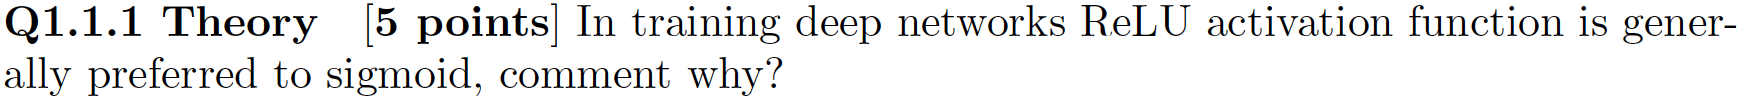
\includegraphics[width=\textwidth]{1_1_1.png}
\end{problem}

\begin{solution}
ReLu function is popular because it is computationally fast without needing to calculate 
the exponential function. But most importantly, ReLu has a benefit over Sigmoid in avoiding
the "vanishing gradient problem". In Sigmoid, If the input $>> 0$, then the output will be saturated 
to 1. If multiple inputs are large, then their corresponding outputs will all
be saturated to 1, and therefore during back propagation, the gradient will be increasingly small. 
This will run into the vanishing gradient problem.
\end{solution}

\begin{problem}[]
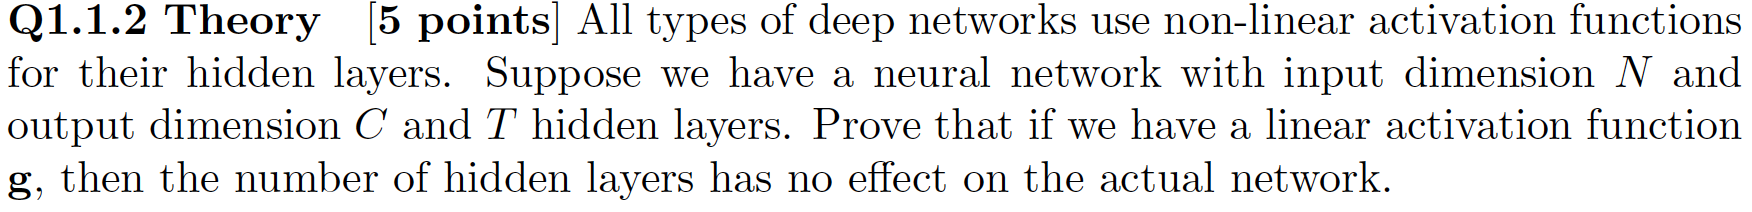
\includegraphics[width=\textwidth]{1_1_2.png}
\end{problem}

\begin{solution}
If we have a linear function $g$, then despite of how many hidden layers we have, all of them 
can be concatinated to be a single linear function since applying linear functions multiple times
will be the same as applying the composite linear function once: $g(x) = y, l(y) = z$ is the same as $
f(x) = g(l(x)) = z$, where $f = (g\circ l)$.

Supposed from the given variables, we have input dimension $N$, output dimension $C$, $T$ hidden layers $H$ of dimension $H_1,H_2, \ldots, H_T$. Also supposed our linear activation functions $g_1, g_2, \ldots, g_T, g_C$, weights $W_1, W_2, \ldots, W_T, W_C$, and biases $b_1, b_2, \ldots, b_T, b_C$, then the output can be calculated by forward propagation as follow:
\begin{align*}
  Output &= g_C(W_C(\ldots(W_2(g_1(W_1\times input+b_1))+b_2))\ldots)b_C)\\
         &= g_C(W_C(\ldots(W_2(g_1(W_1\times input)+ g_C(W_C(\ldots(W_2(g_1(W_1\times b_1))b_2))\ldots)b_C)\\
         &= f(input) + b_f
\end{align*}
This is equal to linearly transform and add to an offset of the input.
\end{solution}
\newpage

\begin{problem}[]
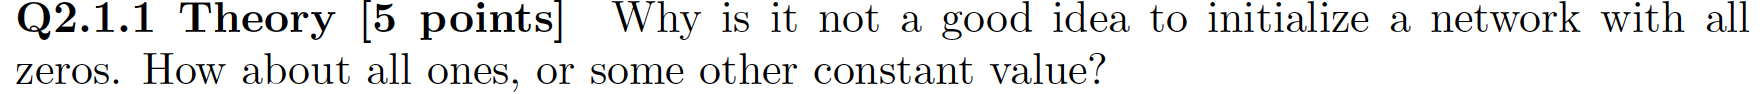
\includegraphics[width=\textwidth]{2_1_1.png}
\end{problem}

\begin{solution}
It is a bad idea to have all the initialial values to be zero or a constant. It is a bad idea because there is a high potential
of running into vanishing gradient problem. Suppose at some layer all the inputs will be outputted the same, and 
at the layer the gradient will be the same and therefore the updates will be the same during parameters update. This runs into a repetition and in effect the layer is deactivated since it simply passes through the parameters with 
all the same values.
\end{solution}

\begin{problem}[]
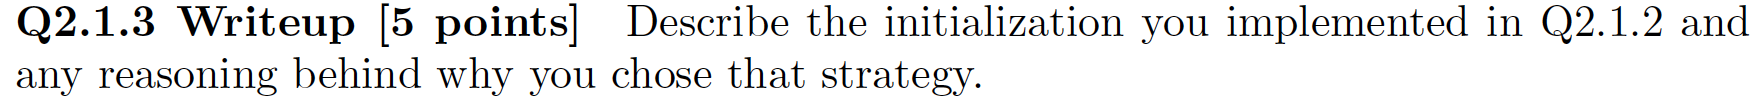
\includegraphics[width=\textwidth]{2_1_3.png}
\end{problem}

\begin{solution}
In Q2.1.2, I have followed the suggestion of "Delving Deep into Rectifiers: Surpassing Human-Level Performance on ImageNet Classification by He et al." which is to initialize the weight by a random value devided by $\sqrt{(2/n)}$, where $n$ is the number of nodes in that particular layer. For biases, I initialize them to be 0, since 
multiple resources online have suggested that 0 can work as well. 
\end{solution}

\begin{problem}[]
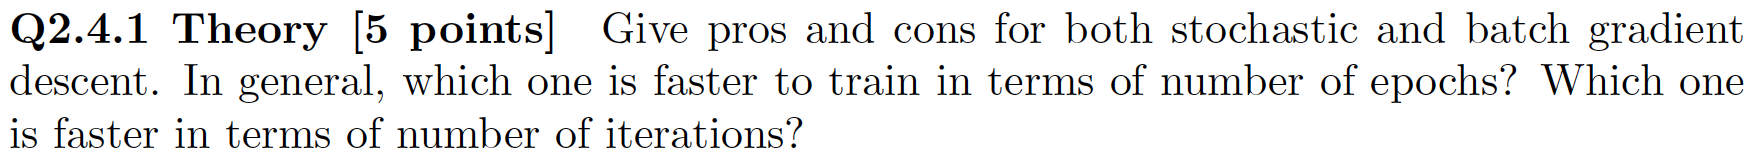
\includegraphics[width=\textwidth]{2_1_4.png}
\end{problem}

\begin{solution}
Stochastic gradient descent runs parameter update after every single sample in an epoch, and therefore, it requires
much more computation time than batch gradient descent, which updates once after all the samples have been run through. However, stochastic gradient descent achieves higher accuracy, requires less computation power than batch gradient descent, and requires less amount of epochs to train since the parameters have been udpated more frequenctly. There is also mini-batch update which updates after a small batch of samples, (usually a few hundred samples). Mini-batch compromises the pros and cons of stochastic and batch gradient descent. 

I implemented stochastic gradient descent update.
\end{solution}
\newpage

\begin{problem}[]
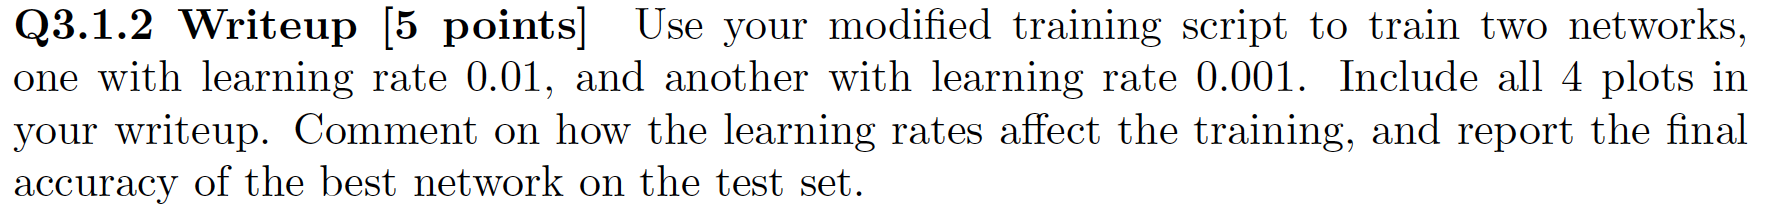
\includegraphics[width=\textwidth]{3_1_2.png}
\end{problem}

\begin{solution}
The results are shown below:\\
leanring rate 0.01:\\
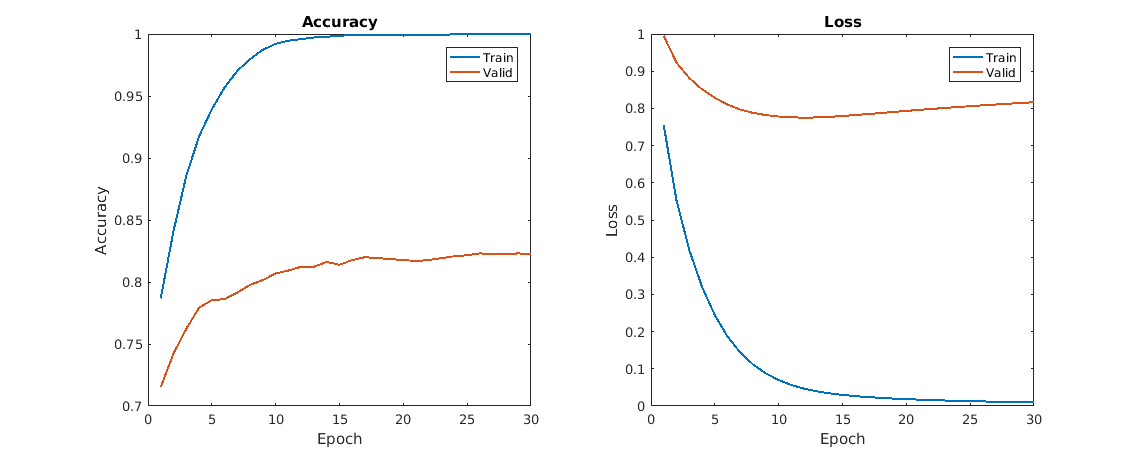
\includegraphics[width=\textwidth]{3_1_2_1.png}\\
learning rate 0.001:\\
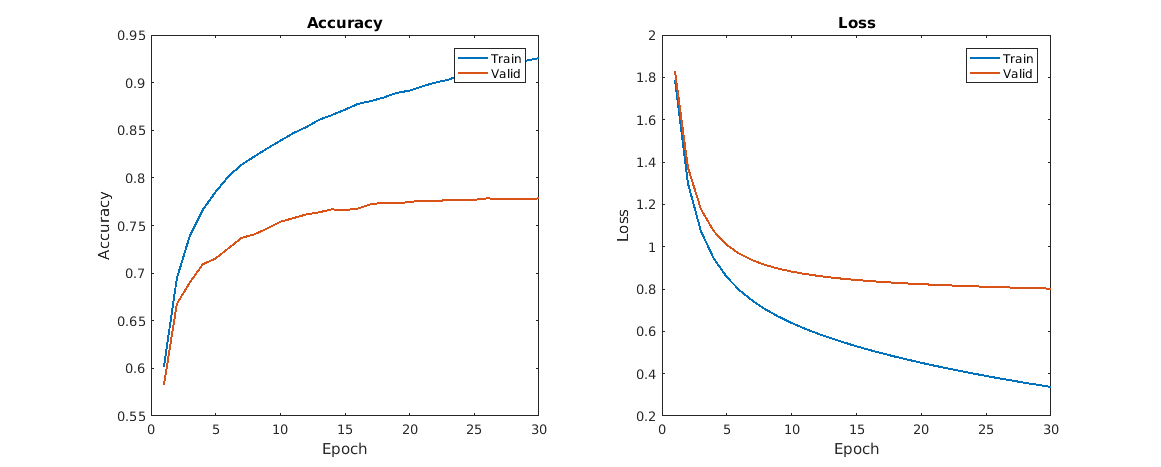
\includegraphics[width=\textwidth]{3_1_2_2.png}\\
From above graphs, we see that the learning rate has sigificantly affect the training: the higher
learning rate, the faster the training goes, and vice versa. However in my implementation, the traning is too fast such
that it overfits the training data. We can tell from the increase in loss of validation data after epoch 12 or so, 
and the 100\% accuracy of training data. Using the parameters of learning rate 0.01, we achieve the accuracy
of  to test set. 
\newpage
The accuracy from learning rate 0.01 is 82.31\%, and the accuracy from learning rate 0.01 is 78.46\%.
The results are also shown in below graphs along with train and validation dataset:\\
0.01:\\
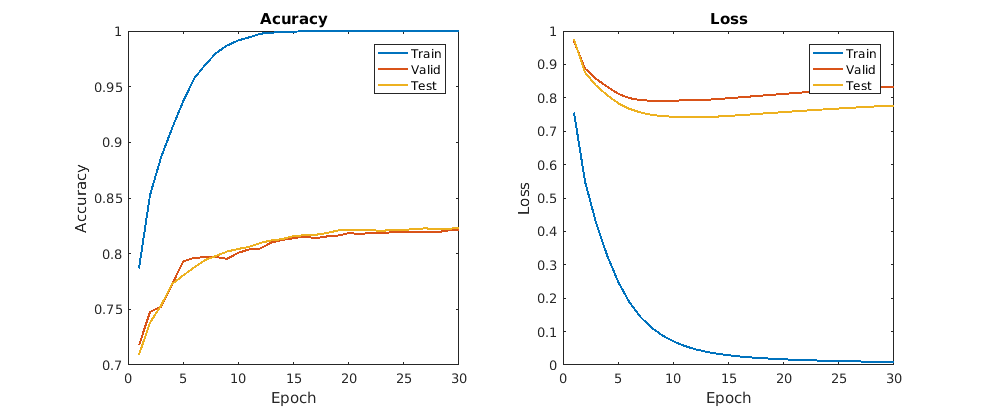
\includegraphics[width=\textwidth]{3_1_2_11.png}\\
0.001:\\
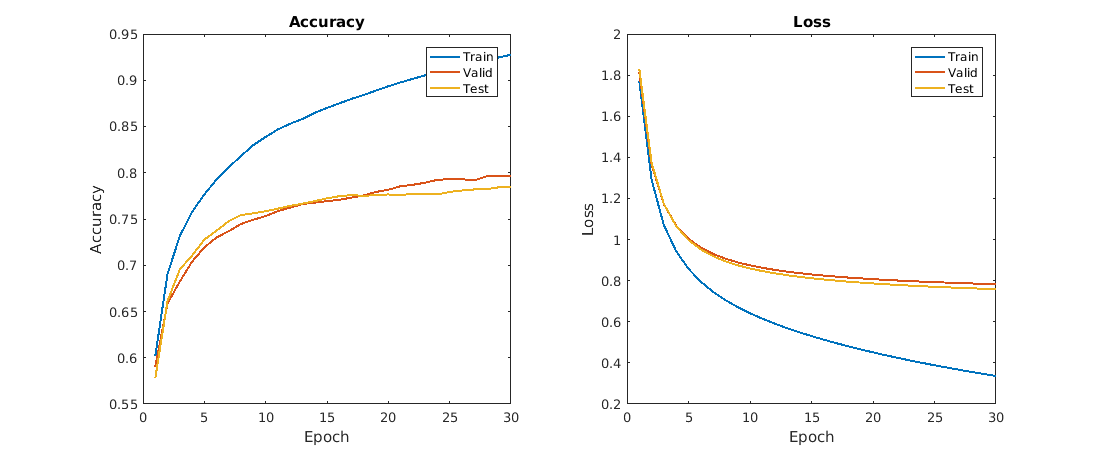
\includegraphics[width=\textwidth]{3_2_1_11.png}


\end{solution}
\newpage

\begin{problem}[]
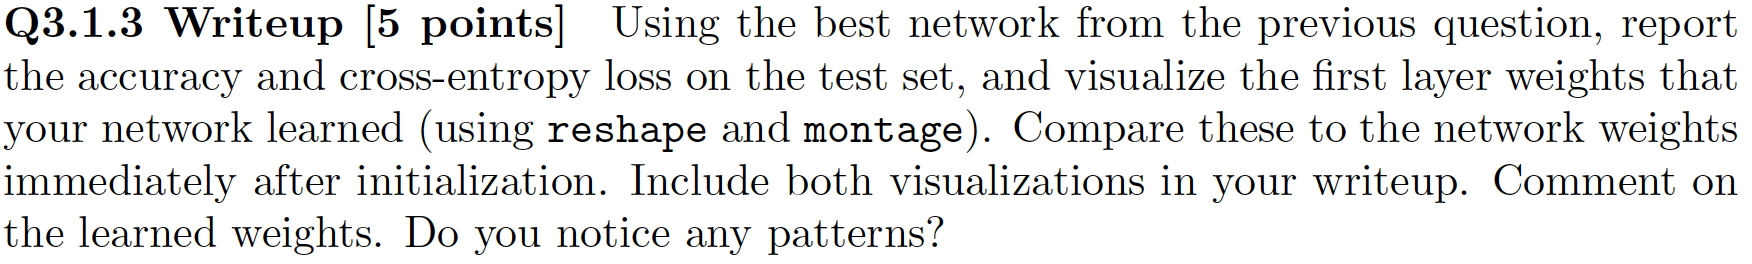
\includegraphics[width=\textwidth]{3_1_3.png}
\end{problem}

\begin{solution}
Accuracy and loss of learning rate 0.01:\\
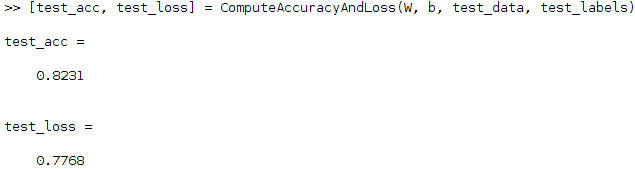
\includegraphics[width=0.8\textwidth]{3_1_2_12.png}\\
Accuracy and loss of learning rate 0.001:\\
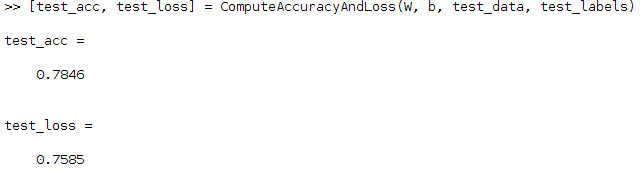
\includegraphics[width=0.8\textwidth]{3_1_2_13.png}\\
The first layer weight immediately after initialization:\\
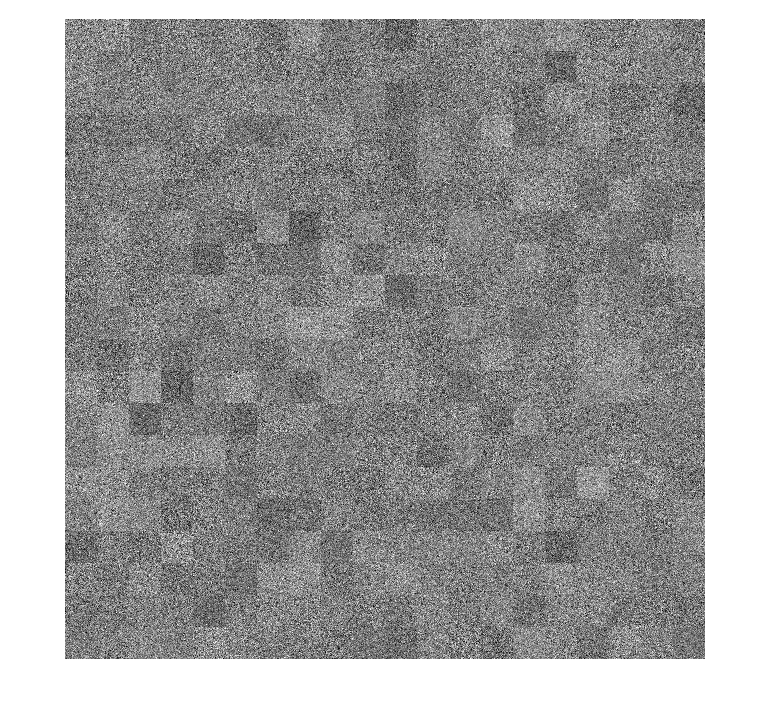
\includegraphics[width=\textwidth]{3_1_3_1.png}\\
Zooming in:\\
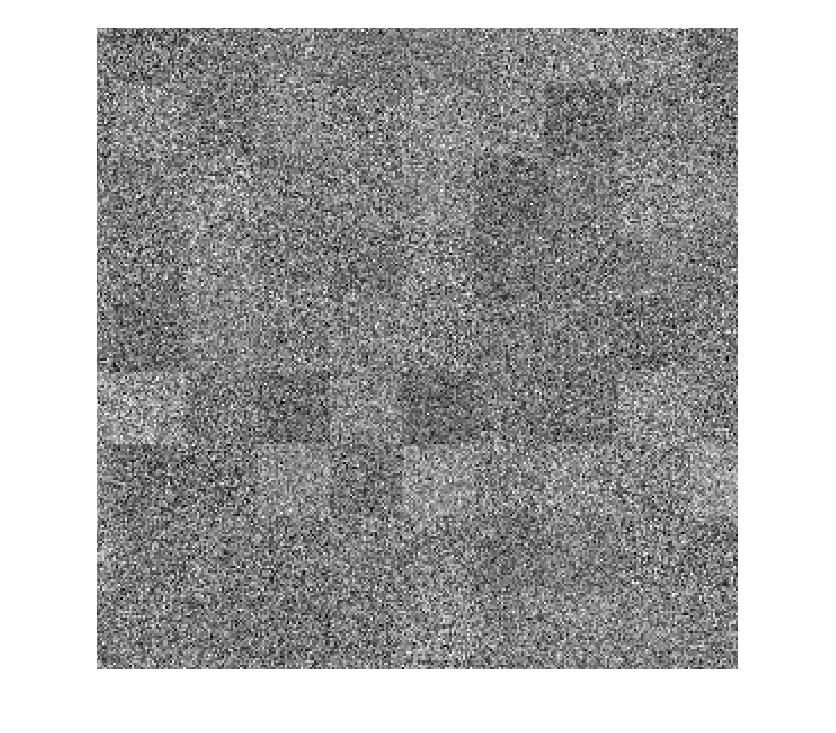
\includegraphics[width=\textwidth]{3_1_3_211.png}\\
\newpage
The first layer weight after 30 epochs:\\
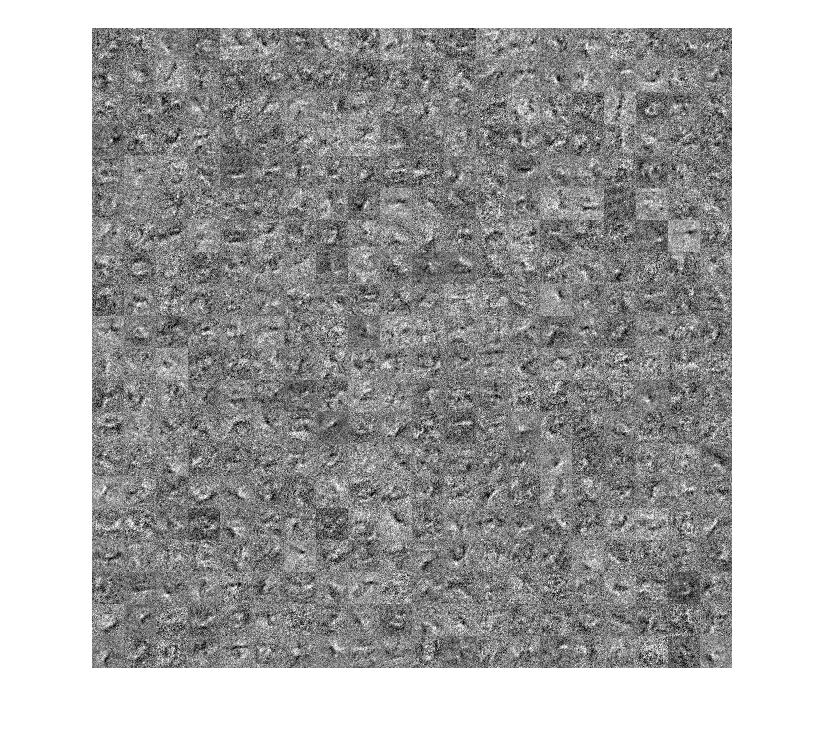
\includegraphics[width=\textwidth]{3_1_3_21.png}\\
Zooming in:\\
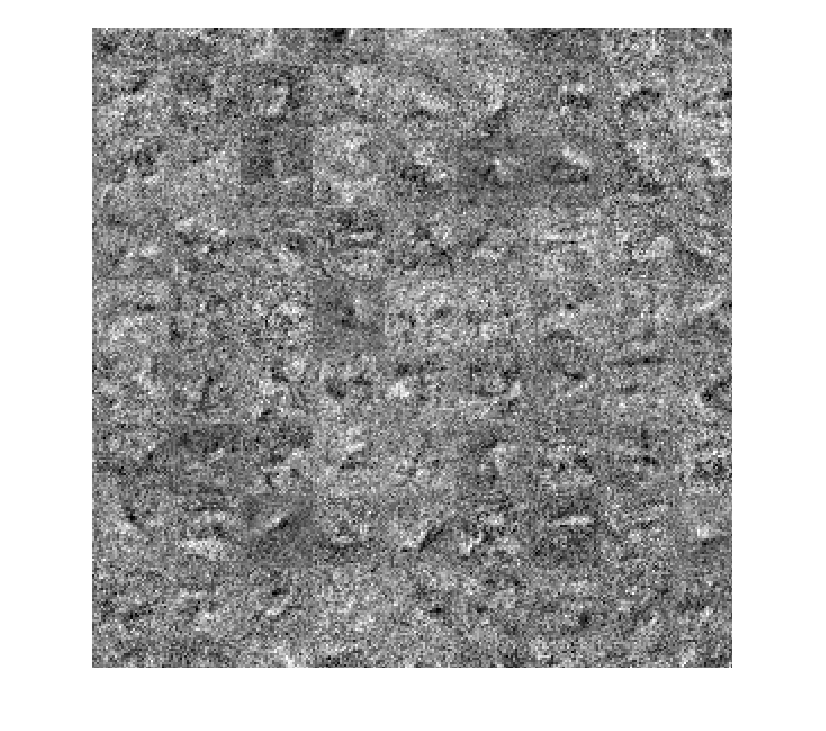
\includegraphics[width=\textwidth]{3_1_3_111.png}\\
As we can see, the weight after initialization doesn't appear to be having any structures, which makes sense
because we randomly initialize the weight. After 30 epochs of training, we can see that the weight at each node
appears to have some structures, such as edge detector, blob detector, or laplacian function. This shows that
during the training, the network has pick up significant features of the training data, and use them to modify
the weights. 
\end{solution}
\newpage

\begin{problem}[]
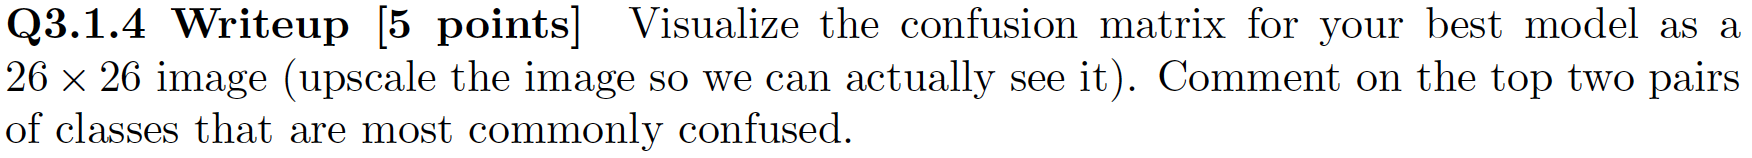
\includegraphics[width=\textwidth]{3_1_4.png}
\end{problem}

\begin{solution}
The confusion matrix is shown below:\\
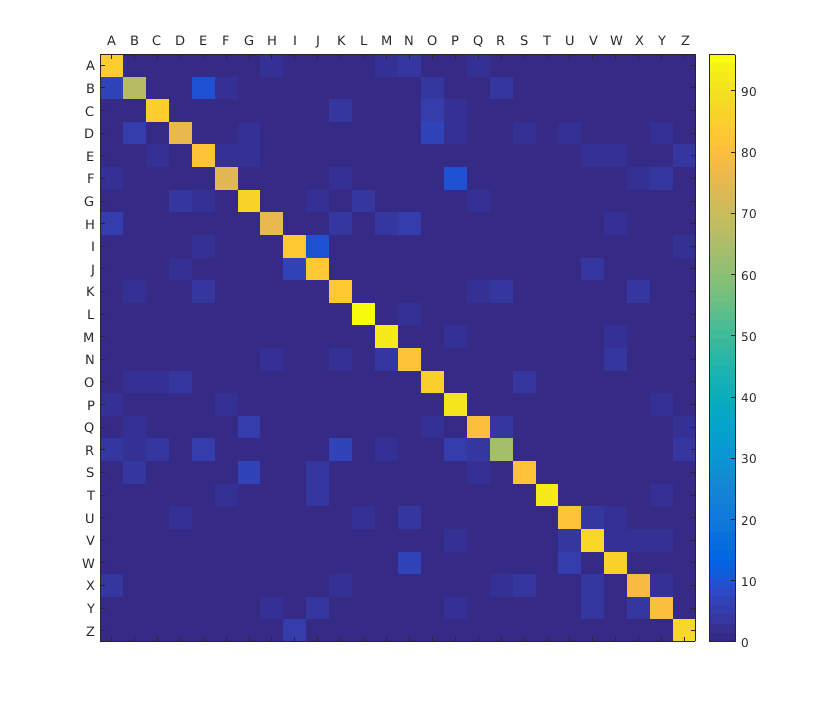
\includegraphics[width=\textwidth]{3_1_4_1.png}\\
As shown, $I$ and $J$ are easily confused because their structure is similar. Other comfusing cases are $F$ and $P$,
$D$ and $O$, $B$ and $E$, which are casese where the structures are also similar, and therefore the network gets 
confused about them.
\end{solution}
\newpage

\begin{problem}[]
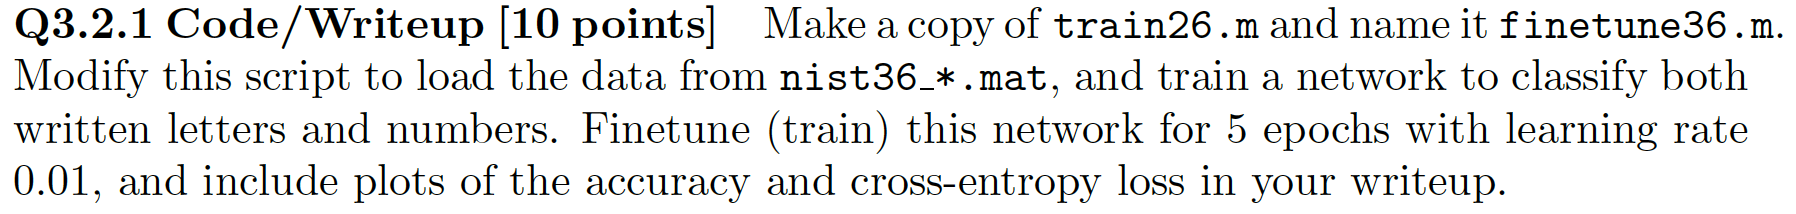
\includegraphics[width=\textwidth]{3_2_1.png}
\end{problem}

\begin{solution}
Loss and accuracy after 5 epochs:\\
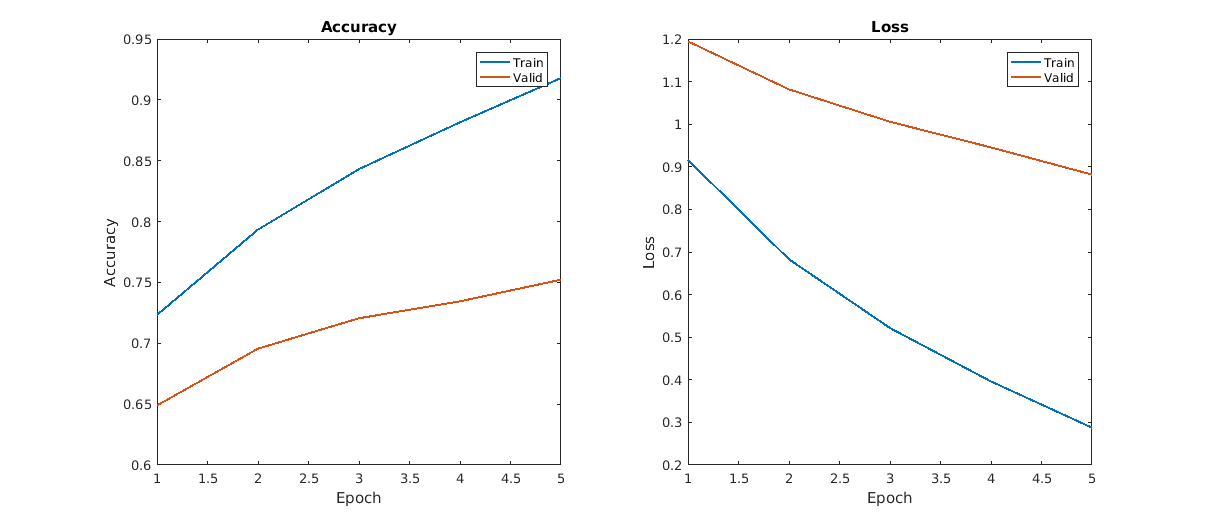
\includegraphics[width=\textwidth]{3_2_1_1.png}\\
Loss and accuracy after 10 epochs:\\
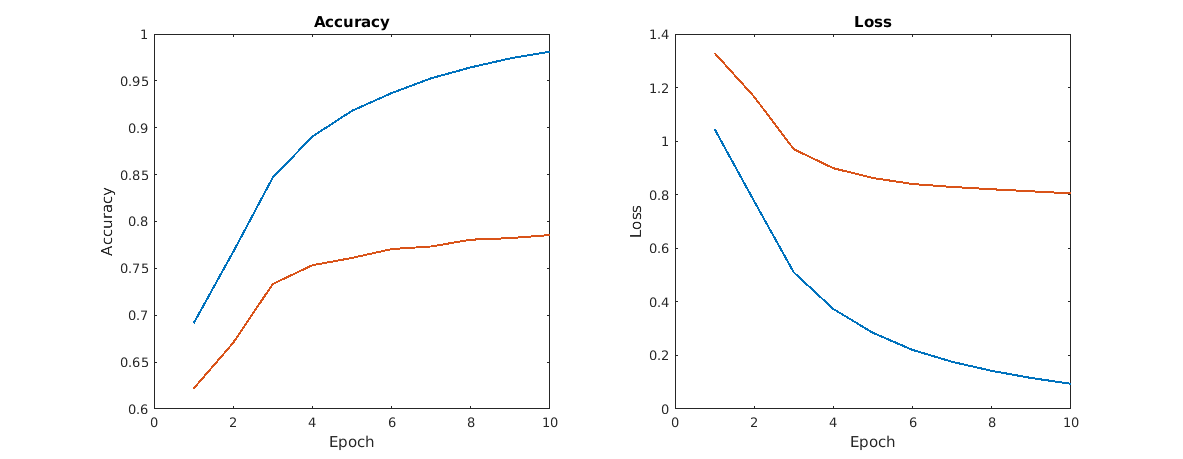
\includegraphics[width=\textwidth]{3_2_1_2.png}\\
\end{solution}
\newpage

\begin{problem}[]
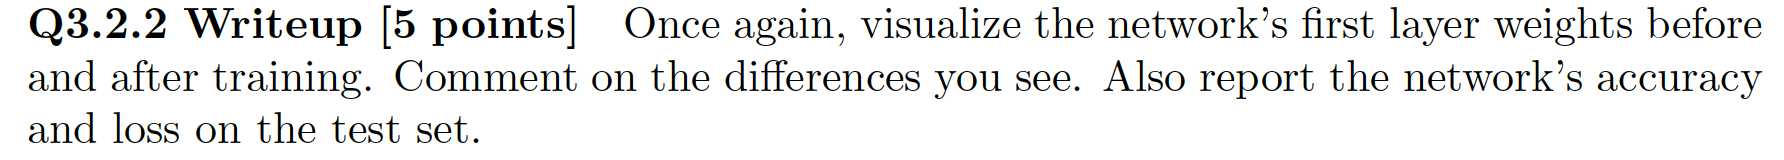
\includegraphics[width=\textwidth]{3_2_2.png}
\end{problem}

\begin{solution}
Test results are shown below:\\
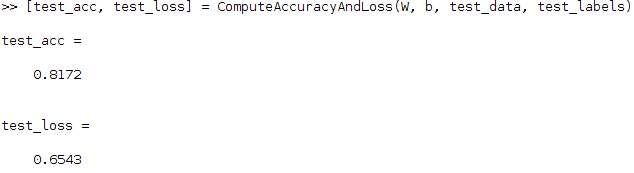
\includegraphics[width=\textwidth]{3_2_2_111.png}\\
The first layer weight immediately after initialization:\\
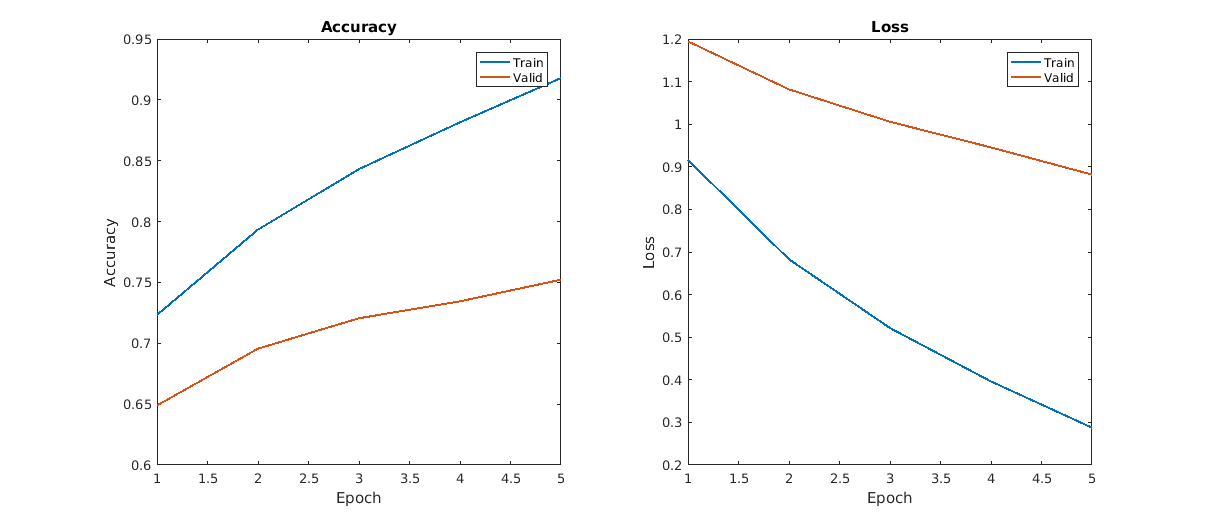
\includegraphics[width=\textwidth]{3_2_2_1.png}\\
Zooming in:\\
\includegraphics[width=\textwidth]{3_2_2_11.png}\\
\newpage
The first layer weight after 5 epochs:\\
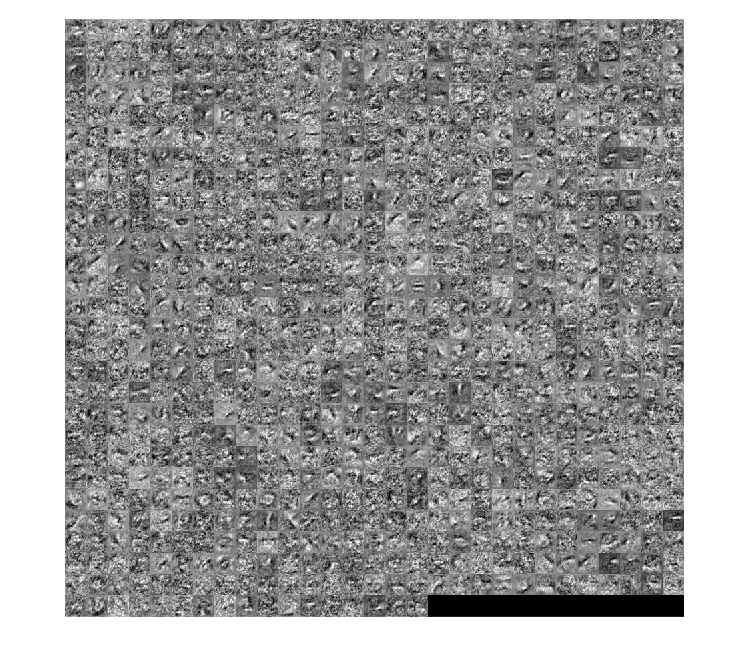
\includegraphics[width=\textwidth]{3_2_2_2.png}\\
Zooming in:\\
\includegraphics[width=\textwidth]{3_2_2_12.png}\\
We can see that both weights show structures, but after the training, there are less "noise" in the 
sense that the strutures become much more apparent. This is because after training, the 
network has enhanced those pre-trained structures.
\end{solution}
\newpage

\begin{problem}[]
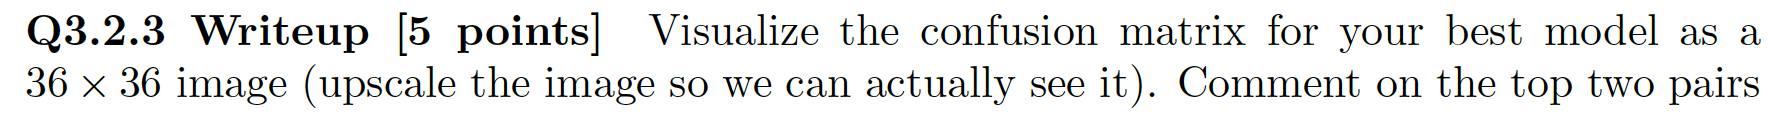
\includegraphics[width=\textwidth]{3_2_3.png}
\end{problem}

\begin{solution}
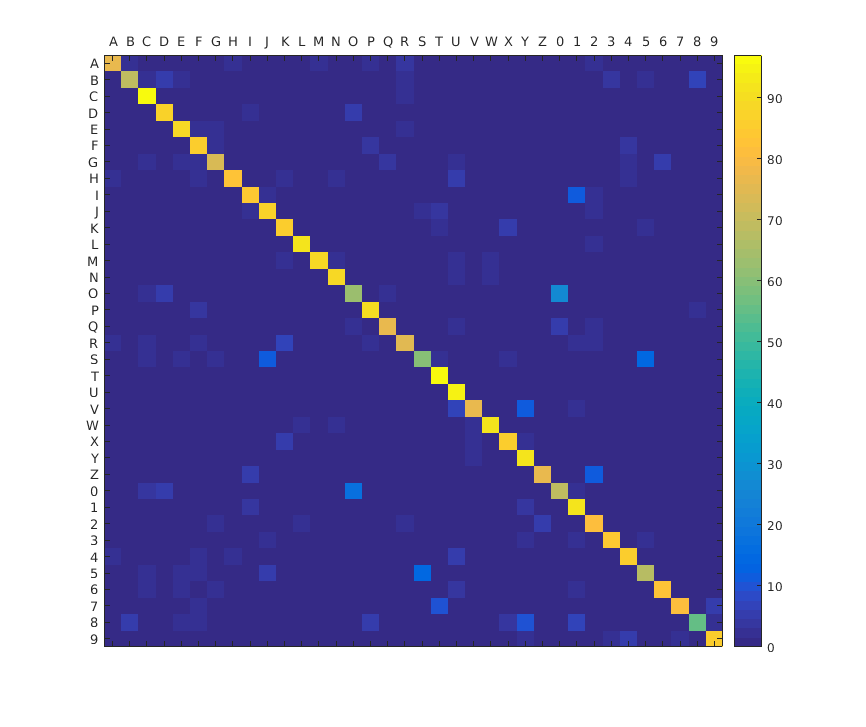
\includegraphics[width=\textwidth]{3_2_3_1.png}
The confusion matrix shows that $0$ and $O$ are easily confused, also $5$ and $S$, $V$ and $Y$. These
characters have similar structures as well.
\end{solution}
\newpage

\begin{problem}[]
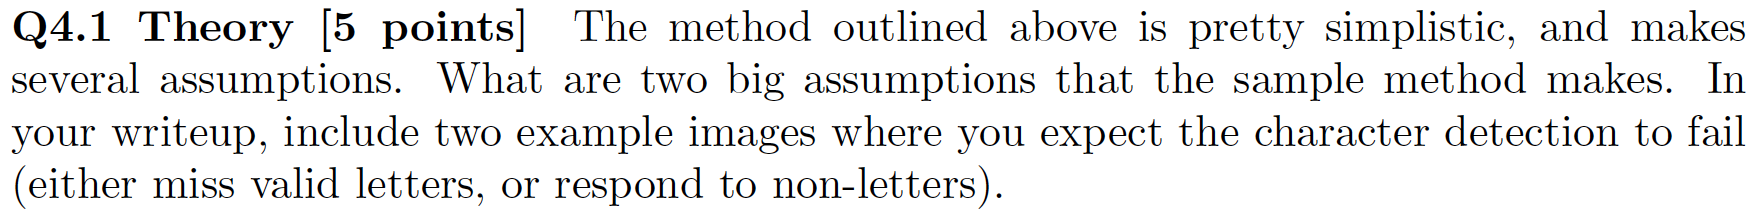
\includegraphics[width=\textwidth]{4_1.png}
\end{problem}

\begin{solution}
The algorithm assumes that each letter is spatially apart, and therefore each letter can
be extracted by itself. It also assumes that the letter has a significant difference in intensity
than the background, with background being clear without noise, so the algorithm can tell the letters from the background using a simple threshold value method. Lastly, the algorithm might assume that each line of text is close to horizontal, so solely using the y-position can it tell the line differences.
\end{solution}
\newpage

\begin{problem}[]
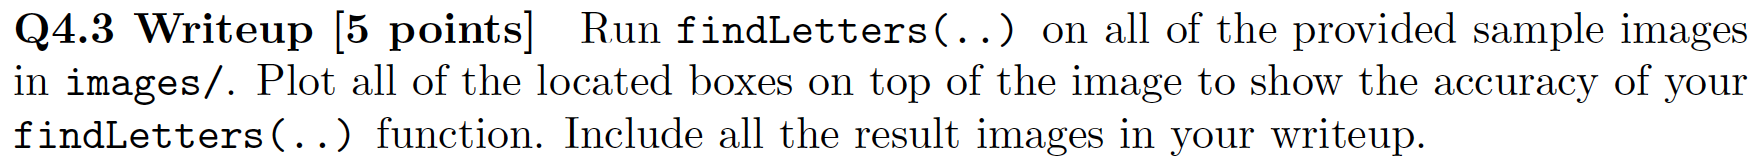
\includegraphics[width=\textwidth]{4_3.png}
\end{problem}

\begin{solution}
The results are shown below, which each color represents different line:\\
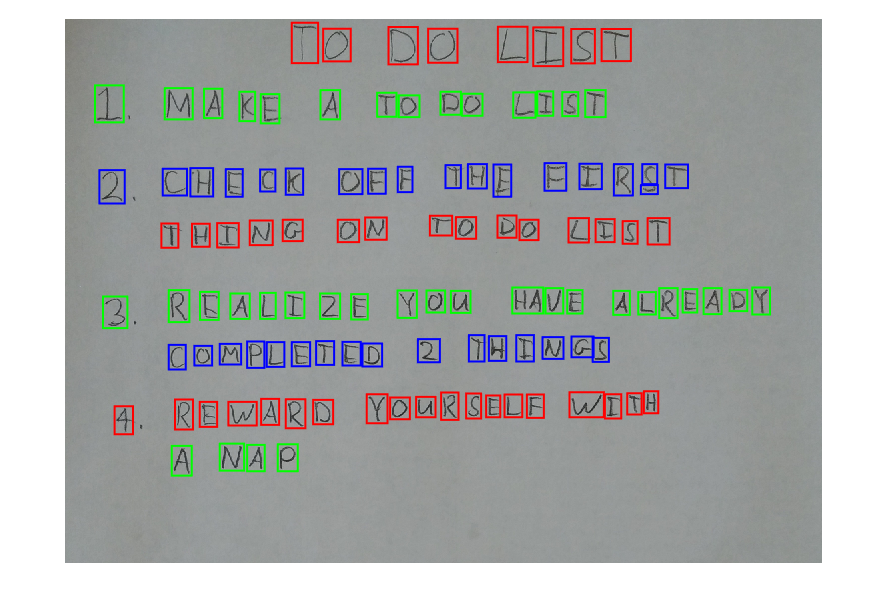
\includegraphics[width=\textwidth]{4_3_4.png}\\
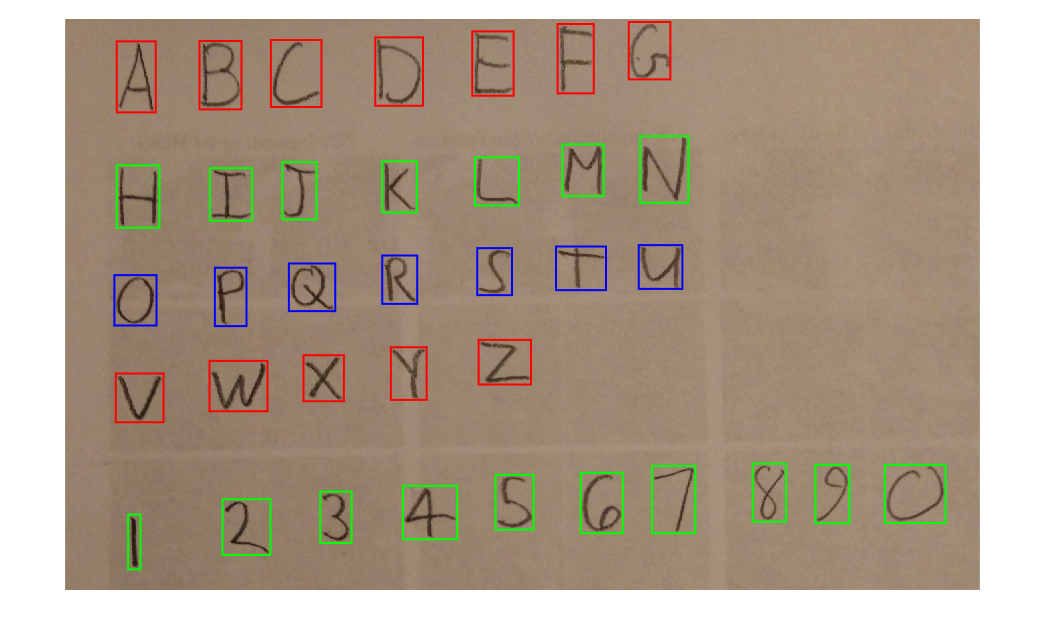
\includegraphics[width=\textwidth]{4_3_3.png}\\
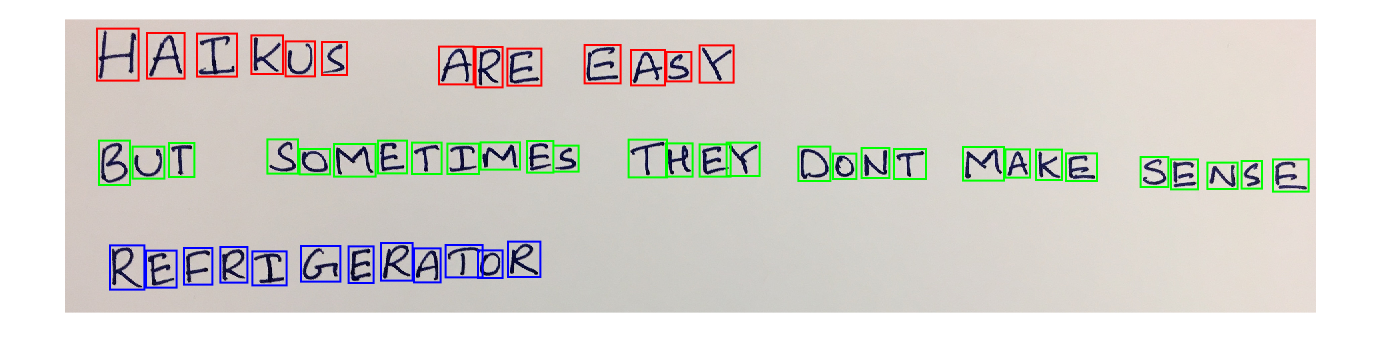
\includegraphics[width=\textwidth]{4_3_2.png}\\
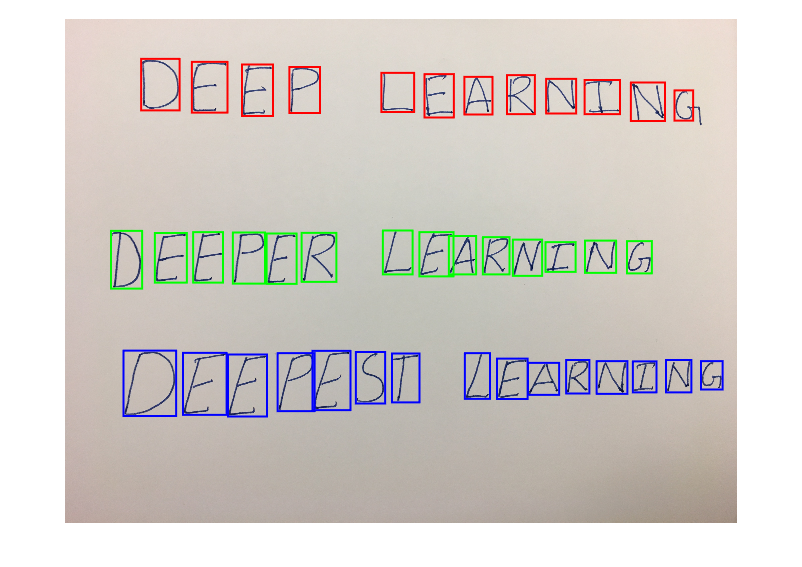
\includegraphics[width=\textwidth]{4_3_1.png}\\
\end{solution}
\newpage

\begin{problem}[]
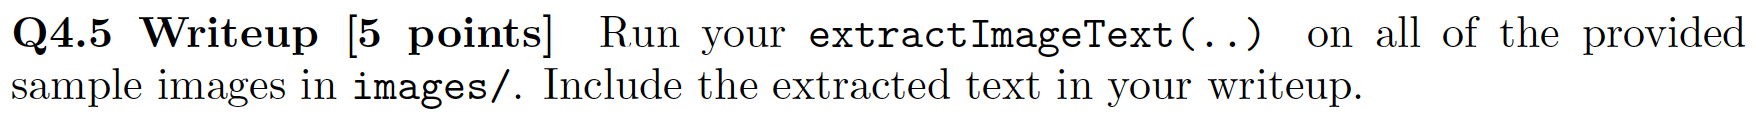
\includegraphics[width=\textwidth]{4_5.png}
\end{problem}

\begin{solution}
The below results are corresponding to the image sequence in the previous questions:\\
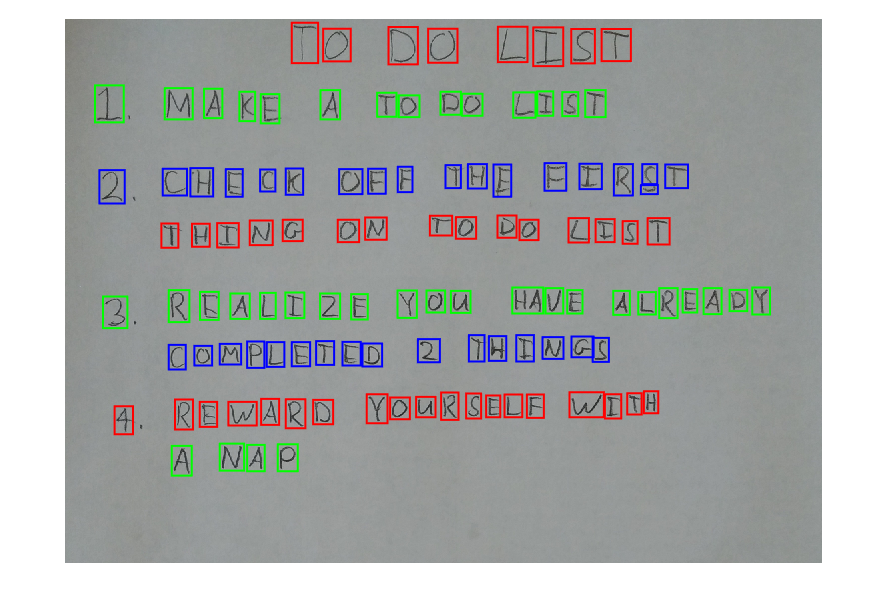
\includegraphics[width=\textwidth]{4_3_4.png}\\
\includegraphics[width=\textwidth]{1.png}\\
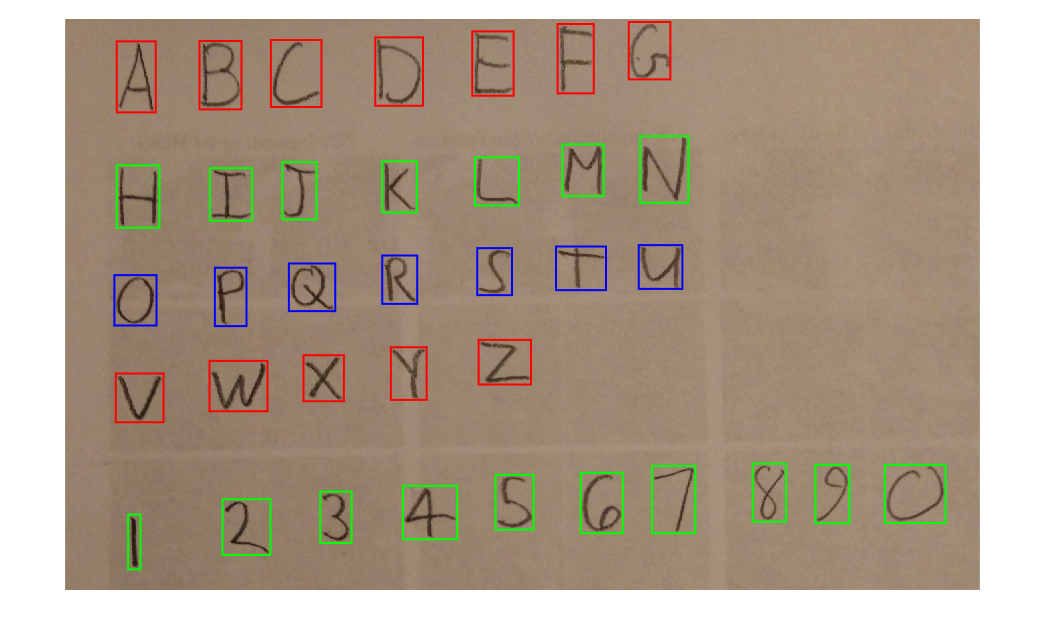
\includegraphics[width=\textwidth]{4_3_3.png}\\
\includegraphics[width=\textwidth]{2.png}\\
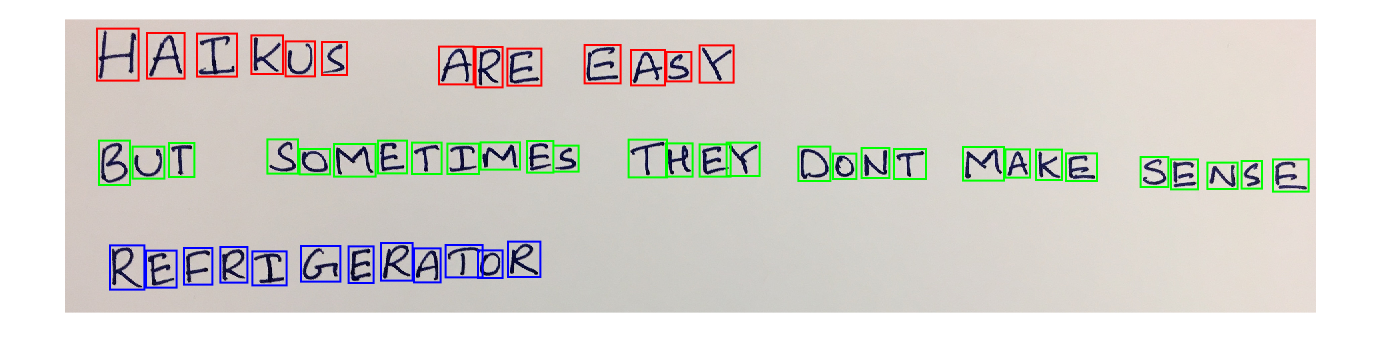
\includegraphics[width=\textwidth]{4_3_2.png}\\
\includegraphics[width=\textwidth]{3.png}\\
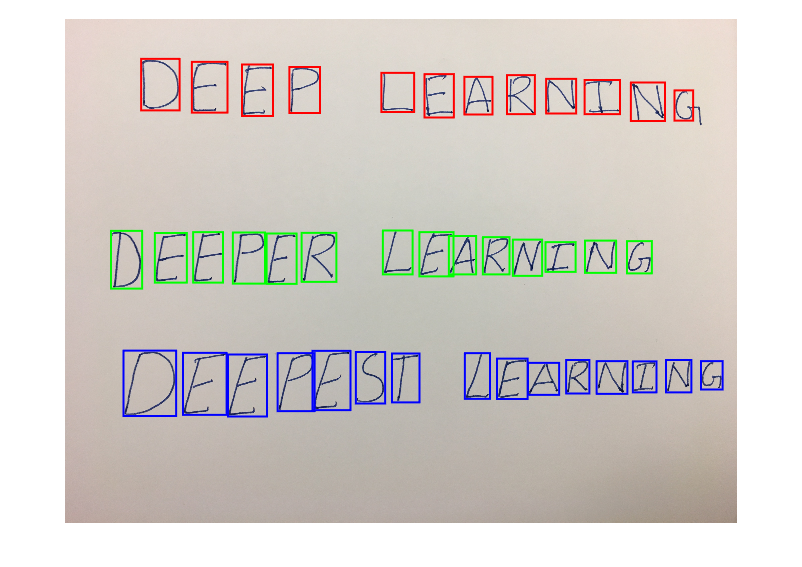
\includegraphics[width=\textwidth]{4_3_1.png}\\
\includegraphics[width=\textwidth]{4.png}\\
As we can see that there are a lot of similar character getting mixed up, such as $0$ and $O$, $I$ and $J$...etc. There
is also problems with 
\end{solution}
\newpage


\end{document}


